\documentclass[b5paper]{report}
\usepackage[lmargin=25mm,rmargin=25mm,tmargin=27mm,bmargin=30mm]{geometry}

\usepackage[toc]{appendix}
\usepackage{graphicx}
\usepackage{subcaption}
\usepackage{listings}
\usepackage{color}
\usepackage{xcolor}
\usepackage{tikz}
\usepackage{hyperref}
\usepackage{parskip}
\usetikzlibrary{positioning,shapes,decorations,calc}

\begin{document}
\title{Concurrent Memory Reclamation on ARM}
\author{Martin Hafskjold Thoresen}
\date{\today}
\maketitle

\newcommand{\note}[1]{{\color{olive}\sffamily #1}}
\newcommand{\todo}[1]{{\color{purple}\sffamily[TODO: #1]}}
\newcommand{\code}[1]{{\ttfamily #1}}

\newcommand{\rustc}{\code{rustc}}
\newcommand{\cargo}{\code{cargo}}
\newcommand{\rustup}{\code{rustup}}



\lstset{ %
 backgroundcolor=\color{white}, % choose the background color; you must add \usepackage{color} or \usepackage{xcolor}; should come as last argument
 basicstyle=\footnotesize\ttfamily,             % the size of the fonts that are used for the code
% breakatwhitespace=false,      % sets if automatic breaks should only happen at whitespace
 breaklines=true,              % sets automatic line breaking
% captionpos=b,                 % sets the caption-position to bottom
 commentstyle=\color{gray},    % comment style
% deletekeywords={...},         % if you want to delete keywords from the given language
% escapeinside={\%*}{*)},       % if you want to add LaTeX within your code
% extendedchars=true,           % lets you use non-ASCII characters; for 8-bits encodings only, does not work with UTF-8
% frame=single,	                % adds a frame around the code
% keepspaces=true,              % keeps spaces in text, useful for keeping indentation of code (possibly needs columns=flexible)
 keywordstyle=\color{purple},    % keyword style
 language=C,                    % the language of the code
 keywords={let,mut,fn,return,pub,struct,where,impl},
% morekeywords={*,...},         % if you want to add more keywords to the set
 numbers=left,                  % where to put the line-numbers; possible values are (none, left, right)
 numbersep=5pt,                 % how far the line-numbers are from the code
 numberstyle=\color{gray}\ttfamily,           % the style that is used for the line-numbers
% rulecolor=\color{black},      % if not set, the frame-color may be changed on line-breaks within not-black text (e.g. comments (green here))
 showspaces=false,              % show spaces everywhere adding particular underscores; it overrides 'showstringspaces'
 showstringspaces=false,        % underline spaces within strings only
% showtabs=false,               % show tabs within strings adding particular underscores
% stepnumber=2,                 % the step between two line-numbers. If it's 1, each line will be numbered
% stringstyle=\color{mymauve},  % string literal style
% tabsize=2,	                  % sets default tabsize to 2 spaces
% title=\lstname                % show the filename of files included with \lstinputlisting; also try caption instead of title
 frame=single,
 rulecolor=\color{lightgray}
}


\begin{abstract}
  \todo{update this!}
  Concurrent programs, like any other program, produces garbage In languages
  that do not have a garbage collector, freeing used memory needs to be
  handled by the programmer, or through other means by the language This
  report compares 3 different memory reclamation schemes: epoch based
  reclamation, hazard pointers, and reference counting We look at how they
  perform when used in different common concurrent data structures, such as
  Queues, Lists, and (probably not) Skip-Lists, on the ARM platform.
\end{abstract}

\chapter{Introduction}
\note{Outline: parallelism, garbage collection, what we are about to do,
rust, performance, usability}

lkajsd

\tableofcontents

\chapter{Background}

\note{I meant to write a quick intro on parallelism, and why we care Maybe this
this is out of scope?}
In 1965 Gordon Moore stated what is now knows as \emph{Moore's Law}, which
roughly states that the number of transistors on integrated circuits will
double every 18 months The law has also been used to describe the clock speed
of central processing units (CPU's) However, this exponential growth came to a
halt during the 2000s, where the clock speed of CPUs stopped between 3 GHz and
4 GHz Over 10 years later high end consumer CPUs still have a clock speed in
that same range, and the performance increase of modern CPUs has mainly been
due to increase in parallelism\note{has it, though Or is it more that CPUs
hasn't really improved that much?} This improvement however, has not been as
noticeable as the former improvements in clock speed. This is because programs
already written cannot automatically use the extra parallelism that newer
architectures give us; Parallelism needs to be accounted for by programmers.

\note{fix this. It reads alright on its own, but the previous paragraph ends
with the same thing, making it very weird to read.}
Despite having multi-core architectures as the most central performance
improvement in CPUs, parallelism is not a success story for programmers Most
mainstream programming languages does not have first class support for parallel
constructs, and synchronization and work management\note{?} must still be
handled explicitly by the programmer, using fairly low level constructs, such
as mutexes and threads \note{what are alternatives?}.
\note{what is the motivation behind this? Do we want to make the claim that
Rust is making low level stuff more approachable, and that we can help
improving the performance of programs written by having CMR in Rust?}
In short, parallelism has yet to be approachable for a lot of programmers.
\note{If we are going to complain on the state of parallel programming we
should at least mention some alternatives.}
\note{Parallelism isn't a success story for programmers Hard, error-prone,
even simple things goes wrong Need effective abstractions to improve this.??}


\subsection*{\note{TODO LIST}}
\note{What do we need to understand in order to appreciate this report?
Moore's law, parallel applications, multi core, blabla\\
Something about ARM.\\
maybe notes on state of the art concurrency stuff?
\\
Notes on memory terminology (retire, reclaim, etc.)
\\
Consider adding MS queue or something to show pitfalls in concurrent programming?
}

\section{Terminology}
We start with basic terminology of memory management Most of the programs we
write \emph{allocate} memory, meaning requesting a memory range from the OS for
exclusive use by the program This memory is then \emph{deallocated}, or
\emph{freed}, when we are done with it, so that the memory may be used at a
later time; the memory is thus \emph{reclaimed} If we want to ``mark'' memory
as freed without freeing it (that is, the program still has exclusive use of
it) we say we \emph{retire} the memory (reasons for doing so will become
apparent) In concurrent settings, we risk accessing memory at the same time;
a \emph{data race} is when multiple threads are operating on the same memory at
simultaneously, and where at least one operation is a write.

Both modern compilers and CPU's may reorder program instructions if they think
it will improve performance, for instance by improving memory locality and thus
improving cache behavior, or reduce pipeline stalling. This may or may not be
acceptable by the program. The guarantee that the instructions executed appear
to take effect in program order is called \emph{sequential consistency}, and
was defined by Leslie Lamport in 1979\todo{source here} We call a system in
which threads can be prevented from making progress \emph{blocking}. For
instance, a system using mutexes is blocking, since a second thread may acquire
the mutex, and be preempted. The opposite of blocking is \emph{non-blocking} A
method is \emph{lock-free} if we have a guarantee that \emph{some} thread will
make progress Note that any given thread may be blocked for an infinite
amount of time For a more thorough introduction see~\cite{herlihy2011art}.


\note{parallel vs concurrent?}


\section{Rust}\label{sec:rust}

\todo{Add note about not a formal spec}
\todo{Add note on generics being like templates and not dyn.disp.}
\todo{destroy/drop}
\todo{Trait terminology. Implements. Mention most important traits?}

% New programming language, memory safety without GC, etc.
\todo{This doesn't read very well. Fix.
This should be written as if you have never heard of Rust, but if you are fairly
familiar with PL terms Worst case, we can refer to the PL book if it goes out
of hand.} Rust is a programming language which focus is safety, speed, and
concurrency It originally emerged from Mozilla Labs in \todo{20??} but is now
freely developed by over \todo{12345} contributors Version 1.0 was released
in May 2015, and the current stable version is 1.21 The language is compiled
and typed, and features type inference and virtually no runtime.

The language differs from most other languages in that it features linear types
by its \emph{ownership} semantics Values are either \emph{owned} or
\emph{borrowed} by its scope When an owned value goes out of scope Rust's
ownership rules guarantees that there are no other references to the object and
it can be safely \emph{dropped} by running its destructor when applicable.
This way the programmer does not have to manually manage memory.

\subsection{A Crash Course in Rust}

Rust's syntax is based on that of C and OCaml Variable bindings are created
with the \code{let} construct, and they are immutable by default, unless marked
with \code{mut} Functions are declared with \code{fn}, and blocks are
surrounded by curly brackets The scope operator is \code{::}.

Almost all syntactic constructs in Rust are expressions, including blocks and
\code{if} statements Expressions terminated by a semicolon have the value of
\emph{unit} (\code{()}) The return value of a function is the value of its
block, which again is the final expression in the block. Alternatively we can
use \code{return}, as in C Similar to C++, Rust programmers prefers
\emph{references} over raw pointers We use \code{\&} and \code{*} as in C and
C++ As with variables, references are immutable by default; the value they
point to cannot be mutated.

\begin{figure}
\begin{lstlisting}[firstnumber=last]
// ERROR:
fn add_five(arg: &u32) { *arg += 5; }
// OK:
fn add_five(arg: &mut u32) { *arg += 5; }
\end{lstlisting}
\end{figure}

Mutable references cannot alias; that is, it is not allowed to have multiple
\code{\&mut} to the same data, and it is not allowed to have one \code{\&mut}
in addition to other references.

References are guaranteed to be valid, through Rusts usage of
\emph{lifetimes} A reference is only allowed to live for as long as the data
it points to This makes it impossible to return a reference to local stack
variable in a function:
\begin{lstlisting}[firstnumber=last]
fn add_five() -> &u32 { let n: u32 = 1; &n } // ERROR
\end{lstlisting}

A central point of Rusts philosophy is to build safe abstractions for
programmers to use For instance, \code{std::box::Box<T>} is a type that heap
allocates a value of type \code{T} The constructor will allocate the memory,
and the destructor will free the memory Since references can never outlive
the value it references, any other pointer to the value is guaranteed by the
compiler to be valid This way we get a safe abstraction over heap allocation.

Through lifetime tracking and the ownership model, Rust avoids the need for a
garbage collector, while still allowing the programmer to not handle memory
management directly. It does however add to the programmers mental overhead,
since lifetime constraints and ownership of the data must be tracked by their
the mental model.

\todo{Mention traits?}
\todo{Add links to The Book ++}
\todo{A longer code example, comparing Rust to C++17?}

\subsection{Rationality behind the rules of Rust}
The rules imposed by Rust might seem overly strict In fact, in the Rust
Survey 2017, $23\%$ of the participants answered that they did not use Rust
because ``Rust is too intimidating, too hard to learn, or too
complicated''\cite{rustsurvey2017} We will see, however, that there are good
reasons for the rules to exist.

The borrowing rules might be the easiest to get the motivation for Since Rust
has no garbage collector, we need to free our allocated memory We must also
ensure that all allocated memory is freed exactly once Borrowing is a natural
solution to this problem. Since a value is only owned at one binding at a time,
we can free memory when the owned binding goes out of scope.

However, ownership alone does not fix use-after-free problems, we need
lifetimes for that Without lifetimes it would be possible to make a reference
to an owned value, and then have the owned value go out of scope and be
dropped, while the reference is still alive in the program. Now the reference
points to freed memory. Lifetimes ensures, statically, that no such references
exists.

Grasping the rationality behind the ``no aliased mutable references'' rule
might be more difficult. Consider the following example: assume we have a
dynamically sized array (\code{Vec}), and that the exclusive mutable reference
does not exist. Now we may have a reference to a value in the \code{Vec}, as
well as a mutable reference to the \code{Vec} itself Consider what happens
when we push a new element into the \code{Vec}; the internal buffer may be
full, so new memory must be allocated, the elements moved over, and the old
buffer is \code{free}d However, this makes the reference to the element
invalid, since the memory it points to is now \code{free}d.

\subsection{Advanced Rust}
\note{Show of why Rust is interesting, eg.\ how the abstractions can be used,
and why it makes sense to look at Rust.}
\todo{Title of the subchapter}
\todo{Ordering of this stuff}
While Rust features rather strict rules for ownership and lifetimes of all
values, the programmer may bend these rules as they wish For instance it is
possible to leak a value by not running its destructor, by using the
\code{std::mem::forget} function, or to explicitly run the destructor of a
value, by calling \code{std::mem::drop}.

The Rust standard library also have \emph{smart pointers}, including reference
counted pointers (\code{std::rc::Rc}), and an \emph{atomic} version
(\code{std::sync::Arc}). \code{Rc} uses a non-atomic counter, and is hence not
safe to share among threads, since it could induce a race condition.
Rust also have \emph{raw pointers}, which behaves like regular pointers in C
and C++ Copying and creating raw pointers are safe operations, but reading a
raw pointer is \code{unsafe}, as there are no guarantee on the memory we are
reading.



\todo{raw pointers, safe abstractions, some other things.}

\note{Finally we should have some examples of all Rust stuff coming together,
so the reader can see why the language as a whole is interesting.
We could also add some stuff about the asm \code{rustc} generates,
demonstrating ``zero-cost abstractions''.}




\section{Parallelism in Hardware}
\note{reconsider having hardware and software sections Maybe it's better to
just have one?} \note{hardware ordering. Atomic operations (CAS, FA, etc.),
notes on other futuristic atomic operations} \note{We should focus on the
things that are currently supported in hardware, since this is more of a
practical thing.} We consider multi-core CPU's with multiple levels of cache;
This includes most modern CPU's, both desktop computers and laptops, as well as
mobile devices such as smartphones and tablets The first cache level, L1, is
usually only used by one core, while the remaining levels, L2 (and maybe L3),
are shared This means that when a program is writing to memory, the same
logical memory may be present in multiple physical locations on the CPU, which
causes synchronization problems when this memory is written to. This is the
problem of \emph{cache coherence}.

\note{???}
We would like our programs to be sequentially consistent However, we also
want our hardware to be performant, and it turns out that these two
requirements are conflicting, and we have chosen the latter.


\todo{could probably make this better: memory models isn't all about
reordering.} Different CPU architectures have different memory models, which
dictates how much the CPU is allowed to reorder reads and writes without
breaking the semantics of the program when ran sequentially For this reason,
architectures have constructs for saying ``do not move memory operations across
this line'', called \emph{memory fences} or \emph{barriers} x86 have a rather
strong memory model, meaning the CPU is very limited in its ability to reorder.
For instance, x86 forbids reads to be reordered with other reads, and writes
with other writes. It also forbids any reordering with locked instructions;
this is very strict, as the preferred instruction used for sequential
consistent atomic store is a locked instruction, meaning atomic stores are full
fences ARM on the other hand, have a comparably weak memory model. A
disadvantage of this is that sequentially consistent atomics require full fences
for both loads and stores, since they are allowed to be reordered ARMv8 fixes
this by having explicit instructions for SC load and store For more
information on x86, see Chapter 8.2.2 in~\cite{intel64}; for information about
ARMv7 and ARMv8 see \todo{sources}.


\note{blabalba}



\section{Parallelism in Software}
\note{Hardware works such and such, but how does programmers handle these
things?  Mention \code{volatile}? Look at instructions?  Many programmers does
not think about cache problems. What about concurrency problems? May they also
be ignored? (no)}

Rust uses the same memory model as LLVM, which is inspired by the C++11 memory
model~\cite{llvmmm}. LLVM also defines the memory ordering constraint types that
Rust uses. We will use the memory orderings as defined in
\code{sync::atomic::Ordering}~\cite{rust-ordering}. There are five variants:
\code{Relaxed}, \code{Release}, \code{Acquire}, \code{AcqRel}, and
\code{SeqCst}, \code{Relaxed} is the weakest and offers no ordering
constraints Atomic operations with this ordering differs only from regular
operations in that the operation is happening instantaneously.
\code{Acquire} and \code{Release} are intended to work in pairs, by loading with
\code{Acquire} and storing with \code{Release} in the same memory location.
\code{Acquire} ensures that data written in between it and a \code{Release}
store on the same memory address is visible to other threads. This is typically
used to implement a lock, where we \code{Acquire} the lock before the critical
section, and \code{Release} the lock after it. Now the operations inside the
critical section are not allowed to be reordered out of it.
\code{AcqRel} is the \code{Release} ordering when used with a store, and
\code{Acquire} when used with a load. \code{SeqCst} is \code{AcqRel}, but it
also guarantees that all threads see all SC operations is the same order.
\note{Maybe we will not use other orderings than SeqCst for anything, for
simplicity?  Time etc. Also, ``Hans Boehm'' warns that it is very hard to get
right, and that it is probably not possible to hide the choices of orderings
from clients of libraries We could write a paragraph here explaining what
it's about, and then just say ``we will stick with \code{SeqCst}.''?}


Modern compilers and CPU's reorder instructions when it improves
performance if they can prove that the end result is the same In sequential
code there is no way to notice the difference Consider
Listing~\ref{lst:reordering}, and assume variables are initialized to 0.
\begin{figure}[ht]
\begin{lstlisting}[caption=Instruction reordering,label=lst:reordering]
// Thread A                     // Thread B
while (f == 0)                  x = 1
  ;                             f = 1
print(x)
\end{lstlisting}
\end{figure}
When ran sequentially (alternating between the two), we would observe no
difference if the assignments were reordered. However, when run concurrently
thread B might decide to assign \code{f = 1} first, and thread A will risk
printing \code{0} instead of \code{1}, which was the only case in the
sequential world.

A solution to this problem is to use a memory fence, in order to explicitly
disallow any reordering past it, as in Listing~\ref{lst:mem-fence}.

\begin{figure}[ht]
\begin{lstlisting}[caption=Memory fence for synchronization,label=lst:mem-fence]
// Thread A                     // Thread B
while (f == 0)                  x = 1
  ;                             fence()
fence()                         f = 1
print(x)
\end{lstlisting}
\end{figure}
However, fences are expensive. We would rather want to just make sure that
there is an ordering relationship between \code{f} and \code{x}. We can obtain
this by using \code{Acquire} and \code{Release} semantics on \code{f}, like in
Listing~\ref{lst:acqrel}. The \code{Release} in Thread B ensures that the
assignment \code{x =1 } is not moved after the store to \code{f}, and the
\code{Acquire} load in Thread A ensures that the access to \code{x} is not moved
above the load of \code{f}. This gives us the desired semantics.
\begin{figure}[ht]
\begin{lstlisting}[caption=Synchronization using orderings,label=lst:acqrel]
// Thread A                     // Thread B
while (f.load(Acquire) == 0)    x = 1
  ;                             f.store(1, Release)
print(x)
\end{lstlisting}
\end{figure}


\section{The ABA Problem}
The ABA problem is one of the most known problems in concurrent programming,
especially within the topic of memory reclamation.
\note{explain what this is about, why it's relevant to MR.}


\chapter{Memory Reclamation}
\note{What is memory reclamation? Why is it hard? What approaches are there?}
\note{Assumed background: had OS, have programmed in C or C++.}

When programming we lend memory from the operating system. This memory must be
returned, or else we will sooner or later run out of it In most modern
programming languages, this is a feature provided by the runtime of the
language We call such languages \emph{managed languages} However, in
languages such as Rust, there is virtually no runtime, so this becomes a
concern of the programmer Garbage collection is typically the name used for
memory reclamation; if we want to pedantic we would say a garbage collector
performs memory reclamation.

In a concurrent setting, we are concerned about the properties of our data
structures, \todo{define this} such as wait-freedom, or lock-freedom.
\todo{rewrite this sentence} One can make the claim that data structures
implemented in managed languages can never obtain some of these properties,
since they depend on the runtime to get execution time in order for the program
to be able to allocate memory Hence, the runtime thread has to get CPU time
in order for the program to make progress \note{Could say this better; the
point is to motivate the usage of Rust.}

The field of concurrent memory reclamation is an active one, and a lot of
different schemes have emerged the recent years. We will look at
\emph{Reference Counting} (RC),
\emph{Epoch Based Reclamation} (EBR),
\emph{Hazard Pointers} (HP),
\note{and maybe a few others?}




\section{Reference Counting}
\todo{this}
Simple, "obvious" solution. But does it work?

\todo{split into two paragraphs? Eventually move history part to bottom, Knuth
style} The idea of reference counting is that we count the number of references
to data, so that we can tell if we are holding the only reference to some
data When we no longer need this reference, we know it is safe to reclaim the
memory the reference points to, since no other reference to that memory
exists Reference counting first appeared in 1960 by G. E.
Collins\cite{collins1960method}, where it was used for collecting nodes of a
linked list The primary downsides of RC is that it is rather expensive, and
that a na\"\i{}ve implementation does not reclaim cycles Today reference
counting is still used, although not in the setting of general memory
reclamation. \todo{source?} \note{Want to say that while RC isn't used in GC,
it is used for other things, like \code{std::rc::Rc} stuff. Also \code{Arc},
even more expensive}.

% TODO: Use this for node drawing, when needed.
%
% \begin{figure}[ht]
% \begin{tikzpicture}
% \tikzset{Node/.style={
%   rectangle split,
%   rectangle split horizontal,
%   rectangle split parts=2,
%   draw,
%   rounded corners=0.1cm
%   }}
%       \node [Node] (A) at (0,0) {\code{Count=3} \nodepart{second} \code{DATA} };\\
%       \node [Node] (B) at (4,0) {\code{Count} \nodepart{second} \code{DATA} };\\
%       \draw[->]  (0.5,-1) -- (0.5,-0.3);
%       \draw[->]  (0,-1) -- (0,-0.3);
%       \draw[->]  (-0.5,-1) -- (-0.5,-0.3);
% \end{tikzpicture}
%   \caption{Data nodes using RC}
% \end{figure}

\todo{Consider adding a code listing instead of using words} Reference counting
is a natural approach to the problem of concurrent memory reclamation The
first observation to make is that we need to use atomic reads and writes to
correctly increment and decrement the reference count. However, the na\"\i{}ve
implementation is not correct Consider two threads operating on some
\code{RC<T>} When thread A want to create a new reference to the data, it
increments the count in the \code{RC} object. Upon destruction, the count is
decremented and the data is freed if the count is 0 However, it is possible
that thread B has a reference to the RC object and that it got preempted right
before incrementing the count Then the whole object gets freed by thread A,
since the count is 0, and when thread B gets execution time again, it has a
pointer to freed memory which it indents to read It is worth noting that we
can free the \emph{data} using this scheme, but not the entire \code{RC} node,
since the \code{count} field may be set to a special value indicating that its
data is freed.

\note{Add note on differential RC:\@
http://www.1024cores.net/home/lock-free-algorithms/object-life-time-management/differential-reference-counting}


% TODO:  Code listing sample here, with custom lineno prefix
%
% \begin{lstlisting}[label=lst:rc-broken,
%                    numberblanklines=false,
%                    % TODO: would like to not copy this all over the place
%                    numberstyle=\color{gray}\ttfamily{}RC]
% node = load_node();
% node.count += 1;
% data = node.data;
% // use the node
% node.count -=1;
% if node.count == 0
%   free(node);
% \end{lstlisting}

\section{Epoch Based Reclamation}
Epoch Based Reclamation (EBR) was introduced by Fraser
in~\cite{fraser2004practical} It is a reclamation scheme based on the
observation that most programs have no references to data structure memory in
between of operations on the structure The time interval in between
operations on the data structure are therefore safe-points (also called grace
periods) for memory reclamation to occur \todo{add something more here}

EBR uses the concept of an \emph{epoch}, a global timestamp which we use to
find out when it is safe to reclaim retired memory The epoch is a global
counter. In addition we have a global list with one entry for each running
thread, which the thread uses for registering the last epoch they read, as well
as whether they are currently performing an operation We call a thread
performing an operation \emph{pinned}, and the action of marking and unmarking
\emph{pinning} and \emph{unpinning} the thread.

When starting an operation a thread reads the global epoch and saves it in its
entry, and pins the thread Upon retiring memory the thread marks the memory
with the global epoch and puts it in a \emph{limbo list} \note{replace with the
three lists instead of marking?} Every once in a while, the threads try to
increment the epoch The epoch can only be incremented if all pinned threads
have seen the current epoch. This way we know that all threads with references
to memory which may be freed by the data structure is either in the current
epoch, or in the previous epoch Lastly, after incrementing an epoch to $e$ we
know that garbage that was added in epoch $e-2$ is safe to be freed.
\note{Should clarify here. Note that the potential counter example is A a wants
to delete X, B incs epoch and reads X, A deletes X, and incs epoch. But, now X
is marked with e+1, even though A was in e, since we're reading the global
epoch on delete.}

\note{Add example from comere?}

There are still a few challenges with EBR A problem is that we are not
allowed to keep references to data across operations, since the thread must be
pinned while we are using the references A natural way to mitigate this
constraint is to leave the thread pinned However, this will stop the
advancement of the global epoch, and thus effectively halting the memory
reclamation An immediate consequence of this is that EBR is not lock-free.
\note{Limits/challenges of EBR. Add more.}

\todo{Add proof? Pseudocode of stuff?}


\section{Hazard Pointers}

Hazard pointers was introduced by Michael in~\cite{michael2004hazard}.
The paper by Michael formalizes hazardous pointers, and includes a proof of
correctness. We will settle for a informal view of them. It is
based on the observation that in most operations on data structure we only need
a small constant number of references to memory that is shared between running
threads. The technique exploits this by allowing each thread to register the
pointers, called \emph{hazard pointers}, the thread wants to use, but which it
cannot be sure are valid. We call such pointers \emph{hazardous}. The number of
pointers we need varies with the algorithm performed, but a typical value is one
or two.

As an example, the $next$ pointers in a linked list would be registered as
hazardous, as they might point to memory that is already removed from the list.
By registering the pointers that are hazardous, other threads can refrain from
changing the referenced data As with RC there are some complications: the
thread might be preempted after reading the hazardous pointer, but before
registering it as hazardous; then another thread may have removed the referenced
data For this reason, we must \emph{validate} the reference after registering
it as hazardous. This can be problematic for structures in which there is no
obvious way of verifying the data. For other structures this is just a matter of
reading a pointer again.

A challenge in usage of HP is that we need to identify which pointers in our
algorithms are hazardous. In comparison, we have no such concerns in EBR, in
which we only need to register memory as garbage when we remove it from the data
structure (we do need to make sure that this memory is only registered by a
single thread) This imposes the choice of memory reclamation onto the
programmer of the data structures using them. In other words, it is unlikely
that HP can be used ``transparently'', in the sense that we can seamlessly
change between, say, HP and EBR\@.

\todo{Revisit RC here, with the stuff from the blog?
Or maybe its better to just put it at the end of the subsection.}


\section{Other Schemes}
\note{We don't have time to implement all interesting schemes,
but it would be nice to have them in the report}


\chapter{Methodology}
\note{How did we implement the schemes? What choices did we have to take?
Whys. Also implementation problems, testing techniques, profiling setup etc.
Include std allocator change}


\section{Implementation}
There is often a disconnect between the idea of a system and the implementation
of that system Algorithms are usually explained at such a high level that a
straight forward implementation in a given language is either impossible,
impractical, or leads to atypical code Programming is more craft than
science, so when implementing a system we must reconsider the system in the
context of the language we are using.

The data structures were first implemented without any regard for memory
reclamation. Allocated memory were simply leaked when no longer needed.


\subsection{Atomics}

\note{Write about atomic types. If this is to be a section we need to clean up
the code in the atomics.rs files. We should probably also look into having HP as
a type in there, instead of doing the handle stuff. Then we can statically check
that hazardous accesses are behind a HP.}

As mentioned in Section~\ref{sec:rust}, it is idiomatic Rust to unitize the type
system in order to help ourselves. We have made other atomic types in addition
to those in the standard library in order to capture wanted semantics.


\subsection{Data Structures}
\label{sec:data-structures}

For comparing concurrent memory reclamation in a meaningful way we need shared
memory, organized in some data structure. We have chosen to implement two of the
most commonly seen concurrent data structures: the Queue and the List. Both
implementation are well known in the field of concurrent data structures. We
chose to implement these relative simple data structures due to time constraints
of the project.


\subsubsection{Queue}

The queue implemented is a Michael-Scott Queue, as described
in~\cite{michael1996simple}. \todo{Consider explaining how the MSqueue works}
The \code{Queue} and \code{Node} structs, as well as the signatures for the
public functions are listed in Listing~\ref{lst:msqueue}. The implementation of
\code{push} and \code{pop} is heavily inspired of the implementation from
Crossbeam\cite{crossbeam-msqueue}.  We support \code{pop\_if}, since we use this
in the implementation of EBR.  \code{push} allocates the memory needed for the
node, which in microbenchmarks have been shown to take the majority of the time:
allocation averaged at 54ns, while the rest of the procedure averaged at 30ns.
A natural optimization of this problem is to allocate nodes from a memory arena
or similar, such that the allocation overhead is amortized over multiple calls
to \code{push}. However, this seriously increses the complexity of the memory
management schemes.

\begin{figure}[ht]
\begin{lstlisting}[caption=Structs for the Michael-Scott
Queue,label=lst:msqueue,numbers=none]
pub struct Node<T> {
    data: ManuallyDrop<T>,
    next: Atomic<Node<T>>,
}
pub struct Queue<T> {
    head: Atomic<Node<T>>,
    tail: Atomic<Node<T>>,
}
impl<T> Queue<T> {
    pub fn new() -> Self;
    pub fn push(&self, T);
    pub fn pop(&self) -> Option<T>;
    pub fn pop_if(&self, Fn(&T) -> bool) -> Option<T>;
    pub fn is_empty(&self) -> bool;
}
\end{lstlisting}
\end{figure}

The \code{ManuallyDrop} type makes sure the data it wraps, in this case
\code{T}, is not automatically dropped when the node is dropped. We would rather
have the receiver of the data drop the values in the queue. \code{ManuallyDrop}
also makes it possible to \emph{do} drop the data. This is used in the
\code{Drop} implementation of the \code{Queue} itself, since we would like the
values in the queue to be cleaned up correctly when the queue is destroyed.

\subsubsection{List}
\note{how did we implement the list?}

The list we have implemented is based on the list presented by Michael
in~\cite{michael2002high}.  The implementation is similiar to the Michael-Scott
Queue in multiple ways.  For instance, we support a \code{remove\_front}
operation, which is almost identical to \code{Queue::pop}. However, the default
insertion operation of the List pushes the inserted element to the beginning of
the list, such that \code{List::insert} and \code{List::remove\_front} has LIFO
semantics. We also support removals for values which are comparable (implements
\code{PartialEq}). \note{assume we have \code{insert\_after} or something.} This
procedure complicates the implementation: consider the list in
Figure~\ref{fig:list-remove}. We want to remove node B, so we swing
\code{A.next} from B to C. However, at the same time, a thread might insert a
new node X in between B and C. When we now change \code{A.next} to \code{C}, we
have removed two items: B and X.

\begin{figure}[ht]
  \begin{subfigure}[b]{\textwidth}
      \centering
      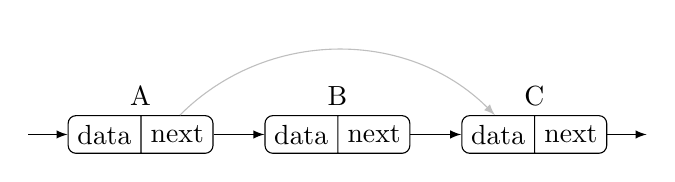
\begin{tikzpicture}
        [node distance = 2.5cm, auto,
        lnode/.style={rectangle split, rectangle split horizontal,
                      rectangle split parts=2, draw, rounded corners=0.1cm }
        ]
        \node [lnode,label={A}] (A)              {\code{data} \nodepart{second} \code{next}};
        \node [lnode,label={B}] (B) [right of=A] {\code{data} \nodepart{second} \code{next}};
        \node [lnode,label={C}] (C) [right of=B] {\code{data} \nodepart{second} \code{next}};
        \draw[-latex] ($ (A.west) - (0.5,0) $) -- (A.west);
        \draw[-latex] (A.east) -- (B.west);
        \draw[-latex] (B.east) -- (C.west);
        \draw[-latex] (C.east) -- ($ (C.east) + (0.5, 0) $);
        \draw[-latex,color=lightgray] ($ (A.north) + (0.5,0) $) to[out=45,in=135] ($ (C.north) -
          (0.5, 0) $);
      \end{tikzpicture}
      \caption{The initial list. When removing B we swing the \code{next}
      pointer over to C.\label{fig:list-remove-a}}
  \end{subfigure}

  \begin{subfigure}[b]{\textwidth}
      \centering
      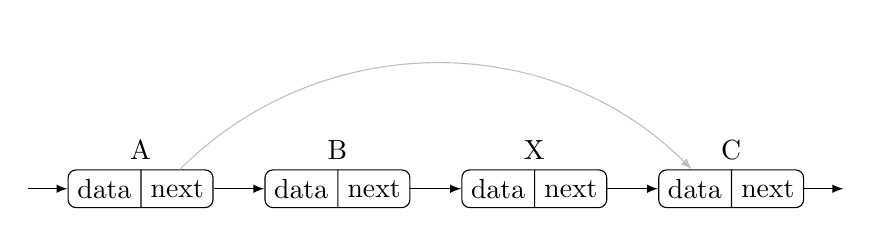
\begin{tikzpicture}
        [node distance = 2.5cm, auto,
        lnode/.style={rectangle split, rectangle split horizontal,
                      rectangle split parts=2, draw, rounded corners=0.1cm }
        ]
        \node [lnode,label={A}] (A)              {\code{data} \nodepart{second} \code{next}};
        \node [lnode,label={B}] (B) [right of=A] {\code{data} \nodepart{second} \code{next}};
        \node [lnode,label={X}] (X) [right of=B] {\code{data} \nodepart{second} \code{next}};
        \node [lnode,label={C}] (C) [right of=X] {\code{data} \nodepart{second} \code{next}};
        \draw[-latex] ($ (A.west) - (0.5,0) $) -- (A.west);
        \draw[-latex] (A.east) -- (B.west);
        \draw[-latex] (B.east) -- (X.west);
        \draw[-latex] (X.east) -- (C.west);
        \draw[-latex] (C.east) -- ($ (C.east) + (0.5, 0) $);
        \draw[-latex,color=lightgray] ($ (A.north) + (0.5,0) $) to[out=45,in=135] ($ (C.north) -
          (0.5, 0) $);
      \end{tikzpicture}
      \caption{Another thread inserts a new node X between B and C.\label{fig:list-remove-b}}
  \end{subfigure}

  \begin{subfigure}[b]{\textwidth}
      \centering
      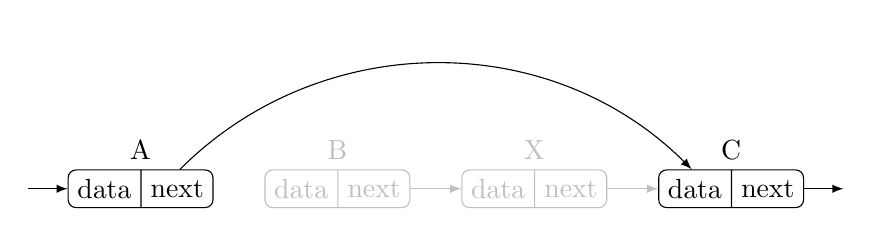
\begin{tikzpicture}
        [node distance = 2.5cm, auto,
        lnode/.style={rectangle split, rectangle split horizontal,
                      rectangle split parts=2, draw, rounded corners=0.1cm }
        ]
        \node [lnode,label={A}] (A)              {\code{data} \nodepart{second} \code{next}};
        \node [lnode,label={\color{lightgray}B},color=lightgray] (B) [right of=A] {\code{data} \nodepart{second} \code{next}};
        \node [lnode,label={\color{lightgray}X},color=lightgray] (X) [right of=B] {\code{data} \nodepart{second} \code{next}};
        \node [lnode,label={C}] (C) [right of=X] {\code{data} \nodepart{second} \code{next}};
        \draw[-latex] ($ (A.west) - (0.5,0) $) -- (A.west);
        \draw[-latex,color=lightgray] (B.east) -- (X.west);
        \draw[-latex,color=lightgray] (X.east) -- (C.west);
        \draw[-latex] (C.east) -- ($ (C.east) + (0.5, 0) $);
        \draw[-latex] ($ (A.north) + (0.5,0) $) to[out=45,in=135] ($ (C.north) -
          (0.5, 0) $);
      \end{tikzpicture}
      \caption{End result. B and X is no longer reachable from the head of the
        list. \label{fig:list-remove-b}}
  \end{subfigure}
  \caption{List removal which removes two elements when there is a concurrent
  insertion. This happens because the \code{compare-and-swap} operation
  performed on \code{A.next} is succeeds since the previous value is not changed.
  However, the new value is logically changed, although there is no way for the
\code{CAS} to detect that.\label{fig:list-remove}}
\end{figure}

Our solution to this problem is simple and effective: we \emph{tag} the node we
want to remove, such that other threads do not add a new node after it. We
exploit the fact that memory addresses are aligned, meaning that the address of
an object in memory is divisible by some number. Objects are typically aligned
by their size, such that \code{u32}s are only on addresses where the four least
significant bits are zero. Bytes are ``aligned'' on 1 byte boundaries,
effectively meaning they are not aligned at all. Since we know that the pointers
we have points to larger objects, the LSB of the pointer itself is free. We use
this to tag the node.
\todo{double check which node we are tagging}
\note{Write about how insert checks for tag. What about searches? Note on search
- if the node is about to be removed, what do we report?}


\subsection{Epoch Based Reclamation}

Our implementation of EBR has both global state and thread local state. The data
in the global state contains three things: the epoch, which is an
\code{AtomicUsize}; a queue of retired garbage, which are tuples of pointers to
memory that we want to free and the epoch when the memory was retired; and a
list of thread markers, \code{List<ThreadMarker>}. This is all stored in the
\code{GlobalState} struct. We use the third-party crate \code{lazy\_static}
which contains a macro for lazy-initialized static variables.  The thread local
data is stored in the \code{LocalState} struct, and is initalized using the
\code{thread\_local!} macro, which is in the Rust standard library. The thread
local data is a pointer to the threads list entry, a counter of how many times
the thread has been pinned, and buffered garbage.

Memory we want to free is hidden behind the \code{Garbage} struct, which
abstracts away the logic of calling the right destructor when we free the
memory. \todo{rewrite this part} This is needed since \code{LocalState::add\_garbage} takes an
\code{Owned<T>}, an owned pointer to any data type. The type information is then
lost for the rest of the garbage pipeline. However, upon destruction we need to
know the type of the data we are dropping. The way we have solved this is by
moving the data to a closure, so that the closure keeps track of the type of the
data.  The closure is never invoked, but upon dropping the closure all of the
values moved to it are dropped. A advanage of this solution is that it is simple
to implement. A disadvantace is that the closure needs to be heap allocated,
which increases the overhead of adding garbage.
\todo{implmeent tags or something, and profile?}

We note that both the thread entry list and garbage queue themselves must be garbage
collected, and that we use EBR on them. This poses a problem: for each
garbage in the list, we need a node. However, that node itself will be garbage
when it is popped from the list, so we need to push it into the garbage list,
which makes a node, etc. Our solution to this is to chunk up garbage in chunks
of a constant size, using the \code{Bag} struct. Thus the garbage queue is a
\code{ebr::queue::Queue<(usize, Bag)>}. The chunking is done thread locally, which also
lowers synchronization overhead, since fewer elements are shared between threads.

When using the collections backed by EBR, we must first obtain a \code{Pin},
which is a proof that the current thread is pinned.  All methods on any
collection requires a pin as the last argument, even though the methods may not
actually use the pin in the method body. There is no way to obtain the pin
directly: users must call the \code{pin} function, and pass in a closure which
is then given the pin as an argument. Listing~\ref{lst:pin-ex} shows example
usage on a queue. This design decision is made in order to discourage users to
grab a pin and keep it for a long amount of time, as this will effectively stop
the memory reclamation. Having a closure also makes it very clear when the
thread stops being pinned. Internally in the \code{ebr} module, there is a
method called \code{Pin::fake}, which makes a pin without actually pinning the
thread. This is an optimization used when we know that we have exclusive access
on certain meomory.

\begin{figure}[ht!]
\begin{lstlisting}[caption=Example usage of the \code{pin} fucntion,
label=lst:pin-ex,numbers=none]
let queue = Queue::new();
pin(|pin| {
  queue.push(42, pin);
});
\end{lstlisting}
\end{figure}

The \code{pin} function is also where we reclaim the memory.  Before calling the
closure passed in, we read the global epoch, and increment our local pin
counter. Every $n$th call to \code{pin}, we try to increment the epoch. For
incrementation to occur, all the pinned threads must have read the current
epoch. If we succeed at incrementing the epoch we also free as much garbage as
allowed from the global garbage list. This scheme is in a sense fair, in that
threads that pin a lot supposedly create a lot of garbage, and these threads
will also have to clean up once in a while. It does however suffer from the fact
that a single thread is set to clean up all the garbage from other threads.
\todo{As i'm writing this, I realize that this is a terrible idea. Should fix.}

The \code{Pin} struct contains a method for retiering garbage, aptly called
\code{add\_garbage}. This method handles the thread local caching of garbage
objects into a \code{Bag}, and pushes the bag with the current epoch into the
global garbage queue when the bag is full. It does not support flushing the
current \code{Bag} (that is, adding it to the global queue even when it is not
full), although this is trivial to implement. \todo{What happends to garbage
when a thread dies? Leak?} Typical useage of \code{add\_garbage} is to make a
node unreachable by its data structure, read the data needed from it, and then
call \code{add\_garbage} with an \code{Owned<Node<T>>}.  \code{pin} and
\code{Pin::add\_garbage} are the only two methods a user of EBR needs to use.

The thread entry list is a potential memory problem: each thread makes an entry
the first time \code{pin} is called, and this entry is never removed. Thus, if
the system keeps creating threads which crashes right after calling \code{pin},
the list will quickly grow, and its elements will never be removed. This problem
can be mitigated by removing the entry from the list if the thread shuts down
gracefully; however this is still a problem if threads crashes. One solution
could be to mark the entries with a timestamp, and remove entries that have been
inactive for too long, as well as to set the threads thread local pointer to
\code{null}. This creates further complications, since thread may have simply
been preempted for a long time, such that other threads think it has crashed.
This problem has not been attempted solved as it is mainly theoretical.

\subsection{Hazard Pointers}

The scheme for hazard pointers is simpler than that of EBR.\@ Each thread have a
\code{ThreadEntry} which contains a fixed size array of hazard pointers, which
are stored as \code{AtomicUsize}. The number of hazard pointers is stored in a
constant. The entries is stored in a global list, and each thread has a local
pointer to its entry in the list.  The \code{Ptr} struct is extended with a
\code{hazard} method, which makes a \code{HazardPtr} struct.  \code{HazardPtr}
wraps an address which, and contains methods for registering and deregistering
the pointer in the threads list, checking if the pointer is registered by other
threads, and a spin-loop for waiting until all other threads have deregistered
the pointer.

Logically, a \code{HazardPtr} is a proof that the pointer is safe to use by the
thread. There is no abstraction around the validation of the hazard pointers;
this has to be done manually. Deregistering the hazard pointer is done in its
destructor.

\note{So far, HPs are freed after spinning. We should probably make a global
queue of retired HPs, and look through them every once in a while. Could use
\code{hazard()} to hijack execution?}





\section{Verification}
Programming concurrent systems is hard Verifying \emph{any} system is also
hard Therefore, we are lead to believe that verifying a concurrent system is
\emph{very} hard This seems to be the case \note{this is probably too dumb
and ``funny''}.

While developing, we used unit tests. See Section~\ref{sec:rust-test} for a
primer on writing tests in Rust.

Testing were primarily done on the development machines of the author, which are
all \code{x86} machines. \todo{add note on bugs on ARM, if any}

The majority of the so-far found bugs in the sytsem is memory bugs. Use after
free bugs, double free bugs, illegal memory accesses, and memory leaks. Double
frees and illegal memory accesses are usually hard faults, such that the
programs execution stops, and we are notified that eg. \code{0x8} is indeed not
a valid memory address to read from.

Use after free bugs and memory leaks are more difficult to find. Here we found
great use in Valgrind\cite{valgrind}, a instrumemtation framework, which
contains the tool \code{memcheck}. \code{memcheck} intercepts all memory
operations, tracks allocations and frees, and is able to report most, if not
all, memory problems. One minor problem with using Valgrind with Rust is that
Valgrind has incomplete support of the default allocator in Rust,
\code{jemalloc}\cite{jemalloc}. However, changing the allocator in Rust to the system
allocator, which Valgrind supports fully, is possible.



\section{Profiling}
\note{How do we benchmark?}
\todo{actually find out this!}

We compare the performance overhead of HP, EBR, and without any reclamation. We
look at their performance implication when we operate on the queue and the list,
as described in Section~\ref{sec:data-structures}. We start out by looking at
the performance on a single threaded system, in order to get a notion of how how
much overhead the schemes impose. Then we look at a larger multithreaded system,
so see how well the schemes handle contention. \note{This sounds like a better
fit for the Results chapter?}

\note{Maybe we want to compare before and after comparisons after we have
optimized the code a little? Look at ordering implications?}

\subsection{Singlethreaded Benchmarks}

An interesting problem that turned up when benchmarking is the following: how do
we benchmark the data structures that does not reclaim any memory? The problem
is that the benchmarking system runs a loop an unspecified number of times, to
make sure the results are statistically significant\note{this is probablyt not
the right word}. This means that we cannot directly control the number of nodes
we allocate which we do not free, and we risk running out of memory. This causes
the system to swap memory to disk, which destroys performance.

Fortunately, \code{bencher} does support executing code in between $n$ benchmark
iterations, where we get to specify $n$. We can use this to preallocate a
\code{Vec}, in which we put pointers to the memory we allocate in the data
structure we profile. Then, after the $n$ iterations, we free that memory.  This
requires some \code{unsafe} code, but it is fully supported by the \code{Vec}
from the standard library. This is a better technique than to allocate the nodes
up front and pass the \code{Node} to the procedures, as this would hide the
allocation cost of the procedure. Listing~\ref{lst:bench-nothing} shows a
benchmark of a Queue using this technique.

\begin{figure}[ht]
  \begin{lstlisting}[caption=Microbenchmark of a data structure without memory
  reclamation,label=lst:bench-nothing]
pub fn push(b: &mut Bencher) {
    const N: u64 = 1024 * 1024;
    b.bench_n(N, |b| {
        let queue = Queue::new();
        let mut ptrs = Vec::with_capacity(N as usize);
        let ptr = ptrs.as_mut_ptr();
        let mut i = 0;
        b.iter(|| {
            queue.push(0usize, unsafe { ptr.offset(i) });
            i += 1;
        });
        unsafe {
            ptrs.set_len(N as usize);
        }
    });
}
  \end{lstlisting}
\end{figure}


\subsection{Multithreaded Benchmarks}


\note{Should add note on microbenchmarks. \code{cargo bench} is alright, but we
get very varying results, since we amortize cleanup over a many runs. This makes
the results given not so good.}


\chapter{Results}
\note{What did we run? Plot some graphs. What did we find out?  Which scheme is
better for which application?  Runtime, power usage, etc.}


\chapter{Discussion}
\note{Whys. How was Rust? Why are the graphs as they are?
What alternatives exists?}

\begin{appendices}
  \chapter{Rust's Toolchain}
  The Rust toolchain consists of multiple tools.
  There is the compiler \rustc{}, the build tool and dependency manager \cargo{},
  and the toolchain manager \rustup.
  \rustup{} is the preferred way of installing Rust\todo{source rustup.rs}.
  \rustup{} also handles cross-compiling, i.e.\ compiling programs for a different
  architecture.

  A major part of Rust's ecosystem is \url{https://crates.io}, the package repository
  for Rust. This is where packages handled by \cargo{} is downloaded from, by default.

  \section{Hello World}
  We show how to install the Rust toolchain on a Unix based system.
  Installing \rustup{} is done by downloading and running an install script from
  \url{https://rustup.rs}:
  \begin{lstlisting}[language=Bash,numbers=none]
% curl https://sh.rustup.rs -sSf | sh
  \end{lstlisting}
  This installs \rustup{}, \cargo{}, and \rustc{}.
  Next we want to use \cargo{} to make a project. This is done by \code{cargo init}.
  \begin{lstlisting}[language=Bash,numbers=none]
% cargo init --bin <name-of-project>
  \end{lstlisting}
  This will create a directory of the name provided, containing two files:
  \code{Cargo.toml} and \code{src/main.rs}.
  The former is the configuration file of the project, which contains:
  metadata such as the project name, version, authors;
  build options such as optimization levels, debug levels, optional flags;
  and dependencies, with versioning and optional flags.
  The initial \code{Cargo.toml} may look like Listing~\ref{lst:cargo.toml}.
  \begin{figure}[ht]
  \begin{lstlisting}[language=,basicstyle=\footnotesize\ttfamily,label=lst:cargo.toml,
  caption=A newly generated \code{Cargo.toml}]
[package]
name = "project-name"
version = "0.1.0"
authors = ["Martin Hafskjold Thoresen <martinhath@gmail.com>"]

[dependencies]
  \end{lstlisting}
\end{figure}
  The other file, \code{src/main.rs} contains the entry point of the program:
  \begin{lstlisting}
fn main() {
    println!("Hello, world!");
}
  \end{lstlisting}

  To run the program, we use \cargo{}:
  \begin{figure}[ht]
  \begin{lstlisting}[language=Bash,numbers=none]
% cargo run
   Compiling project-name v0.1.0 (file:///<path>/)
    Finished dev [unoptimized + debuginfo] target(s) in 0.68 secs
     Running `target/debug/project-name`
Hello, world!
%
  \end{lstlisting}
\end{figure}

  Cargo supports a project to build multiple executables, or no executables at all.
  For more information about cargo see~\url{http://doc.crates.io/index.html}.

  \section{\code{\#[test]} and \code{\#[bench]}}
  \label{sec:rust-test}
  The Rust toolchain supports both testing and benchmarking. To write tests we
  make an inline module named \code{test}, and conditionally compile it using
  \code{\#[cfg(test)]}. This makes the code to be ignored unless we are running
  the tests; this is done with \code{cargo test}. Listing~\ref{lst:cargo-test}
  shows an example test on a \code{Queue}. This is usually put in the same file
  at the \code{Queue} but this is only by convention, and not required.

  \begin{figure}[ht!]
  \begin{lstlisting}[label=lst:cargo-test,caption=An example test in Rust]
#[cfg(test)]
mod test {
    use super::*;
    #[test]
    fn queue() {
        let mut queue = Queue::new();
        queue.push(1);
        queue.push(2);
        assert_eq!(queue.pop(), Some(1));
        assert_eq!(queue.pop(), Some(2));
    }
}
    \end{lstlisting}
  \end{figure}
  The output of \code{cargo test} might look like
  Listing~\ref{lst:cargo-test-output}.
  \begin{figure}[ht!]
    \begin{lstlisting}[label=lst:cargo-test-output,caption=Sample output of
    \code{cargo test},language=,numbers=none]
running 47 tests
test ebr::atomic::tests::valid_tag_i8 ... ok
test ebr::atomic::tests::valid_tag_i64 ... ok
test ebr::bench::pin ... ok
test ebr::queue::bench::push ... ok
test ebr::queue::test::can_construct_queue ... ok
test ebr::queue::test::is_unique_receiver ... ok
    \end{lstlisting}
  \end{figure}

  \todo{Replace this with using \code{bencher}.}
  Benchmarking is similar, except that we do not have a conditional compilation
  flag for benchmarks. For similarity, we can put benchmarks in the \code{bench}
  module. Benchmarks are annotated with \code{\#[bench]}. The benchmarks are ran
  with \code{cargo bench}, which runs all benchmark annotated functions.
  Listing~\ref{lst:bench-test} shows a sample benchmark, and
  Listing~\ref{lst:bench-test-output} shows sample output from a benchmark.
  Note that the benchmark system is not in stable Rust, so we need to use the
  nightly version. The code that is benchmarked is the closure passed to
  \code{test::Bencher::iter}.
  \begin{figure}[ht!]
  \begin{lstlisting}[label=lst:bench-test,caption=An example benchmark in Rust]
mod bench {
    extern crate test;
    use super::Queue;
    #[bench]
    fn push(b: &mut test::Bencher) {
        let q = Queue::new();
        b.iter(|| {
            ::ebr::pin(|pin| {
                q.push(1, pin);
            });
        });
    }
}
    \end{lstlisting}
  \end{figure}
  \begin{figure}[ht!]
    \begin{lstlisting}[label=lst:bench-test-output,caption=Sample output of
    \code{cargo bench},language=,numbers=none,basicstyle=\footnotesize]
test ebr::bench::pin               ... bench:   18 ns/iter (+/- 0)
test ebr::queue::bench::push       ... bench:   57 ns/iter (+/- 12)
test hp::list::bench::remove_front ... bench:    2 ns/iter (+/- 0)
    \end{lstlisting}
  \end{figure}





  \section{Setup for cross-compilation}
  Other targets may be installed through \rustup{}. For instance, if we want to
  make \code{aarch64-unknown-linux-gnu} available for cross-compilation we would run
  \begin{lstlisting}[language=Bash,numbers=none]
% rustup target add aarch64-unknown-linux-gnu
  \end{lstlisting}
  We can either pass in the target architecture to \cargo{} at each invocation,
  or we can configure \cargo{} to use another target by default. We show the latter.
  We make a new file in the project directory called \code{.cargo/config}
  containing Listing~\ref{lst:cargo/config}
  \begin{figure}[ht]
  \begin{lstlisting}[language=,
                     basicstyle=\footnotesize\ttfamily,
                     label=lst:cargo/config,
                     caption=Cargo configuration file for cross-compiling]
[build]
target = "aarch64-unknown-linux-gnu"

[target.aarch64-unknown-linux-gnu]
linker = "aarch64-linux-gnu-gcc"
  \end{lstlisting}
  \end{figure}
  This sets the default target to be \code{aarch-unknown-linux-gnu},
  and specifies the linked to be used.
  After this \code{cargo build} builds for the specified target.
  The executable can be found in \code{./target/aarch-unknown-linux-gnu/debug/}
  with the name of the project.



  \todo{Consider add a Git appendix, to show simple checkout stuff, such that
  ``readers'' who don't know Git can clone the repo, and checkout a commit in
  order to run some tests.}

\end{appendices}

\bibliographystyle{acm}
\bibliography{sources}

\end{document}
